%% Copernicus Publications Manuscript Preparation Template for LaTeX Submissions
%% ---------------------------------
%% This template should be used for copernicus.cls
%% The class file and some style files are bundled in the Copernicus Latex Package, which can be downloaded from the different journal webpages.
%% For further assistance please contact Copernicus Publications at: production@copernicus.org
%% http://publications.copernicus.org/for_authors/manuscript_preparation.html
%% Please use the following documentclass and journal abbreviations for discussion papers and final revised papers.

\documentclass[acp, manuscript]{copernicus} % single column manuscript: used for both discussion and submission

% shortcut commands for one or two column figures
%\newcommand{\igone}[1]{\includegraphics[width=8.3cm]{#1}}
%\newcommand{\igtwo}[1]{\includegraphics[width=12.0cm]{#1}}

\begin{document}
\title{Supplementary}

% \Author[affil]{given_name}{surname}
\Author[1]{Jesse W.}{Greenslade}
\Author[2,3]{Simon P.}{Alexander}
\Author[4,5]{Robyn}{Schofield}
\Author[1,6]{Jenny A.}{Fisher}
\Author[2,3]{Andrew K.}{Klekociuk}

\affil[1]{Centre for Atmospheric Chemistry, School of Chemistry, University of Wollongong}
\affil[2]{Australian Antarctic Division, Hobart}
\affil[3]{Antarctic Climate and Ecosystems Co-operative Research Centre, Hobart, Australia}
\affil[4]{School of Earth Sciences, University of Melbourne}
\affil[5]{ARC Centre of Excellence for Climate System Science, University of New South Wales}
\affil[6]{School of Earth \& Environmental Sciences, University of Wollongong}

\runningtitle{Southern Hemisphere stratospheric ozone intrusions}
\runningauthor{Greenslade et al.}
\correspondence{Jesse Greenslade (jwg366@uowmail.edu.au)}

\received{}
\pubdiscuss{} %% only important for two-stage journals
\revised{}
\accepted{}
\published{}

%% These dates will be inserted by Copernicus Publications during the typesetting process.
\firstpage{1}
\maketitle


% Make figures and tables start with S
\setcounter{table}{0}
\renewcommand{\thetable}{S\arabic{table}}%
\setcounter{figure}{0}
\renewcommand{\thefigure}{S\arabic{figure}}%
\setcounter{section}{0}
\renewcommand{\thesection}{S\arabic{section}}


\section{Weather and Smoke analysis}
  \label{sec:WeatherSmoke}
  
  \begin{figure}[t]
      % Figure 5
      %Figure created in shared HPC folder by egplotday.py in AIRS CO data folder
      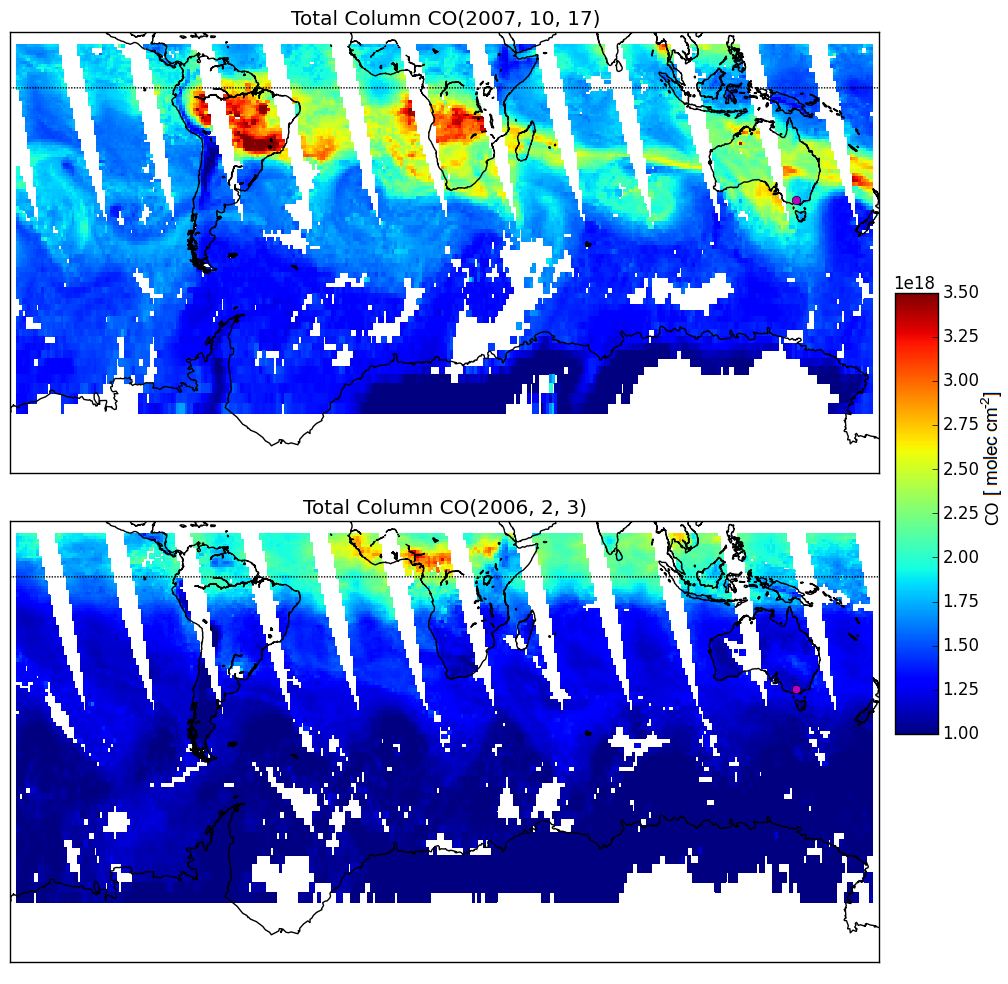
\includegraphics[width=12cm]{../figures/AIRS_compare.png}
      \caption{ %
	Example detection of biomass burning influence using AIRS total column CO. 
	The top panel (17 October 2007) shows a day when ozone above Melbourne (purple dot) could have been caused by a transported biomass burning plume, and so was flagged in subsequent analysis.
	The bottom panel (3 February 2006) shows a day when Melbourne ozone was not influenced by transported smoke.}
      \label{fig:excludedeg}
    \end{figure}

    Figure \ref{fig:excludedeg} contrasts two days; one with and one without signs of biomass burning influence near the Melbourne site (purple circle).
    On 17 October 2007 (top) elevated CO suggests the site may have been influenced by long-range transport from African and/or South American biomass burning.
    In contrast, on 3 February 2006 (bottom) CO columns across the SH show no influence from biomass burning.
    
    \begin{figure*}[t]
    % Figure 5 (discussion version)
    % these IMAGE CREATED BY show_profile.py, EDITTED IN INKSCAPE and then PINTA
      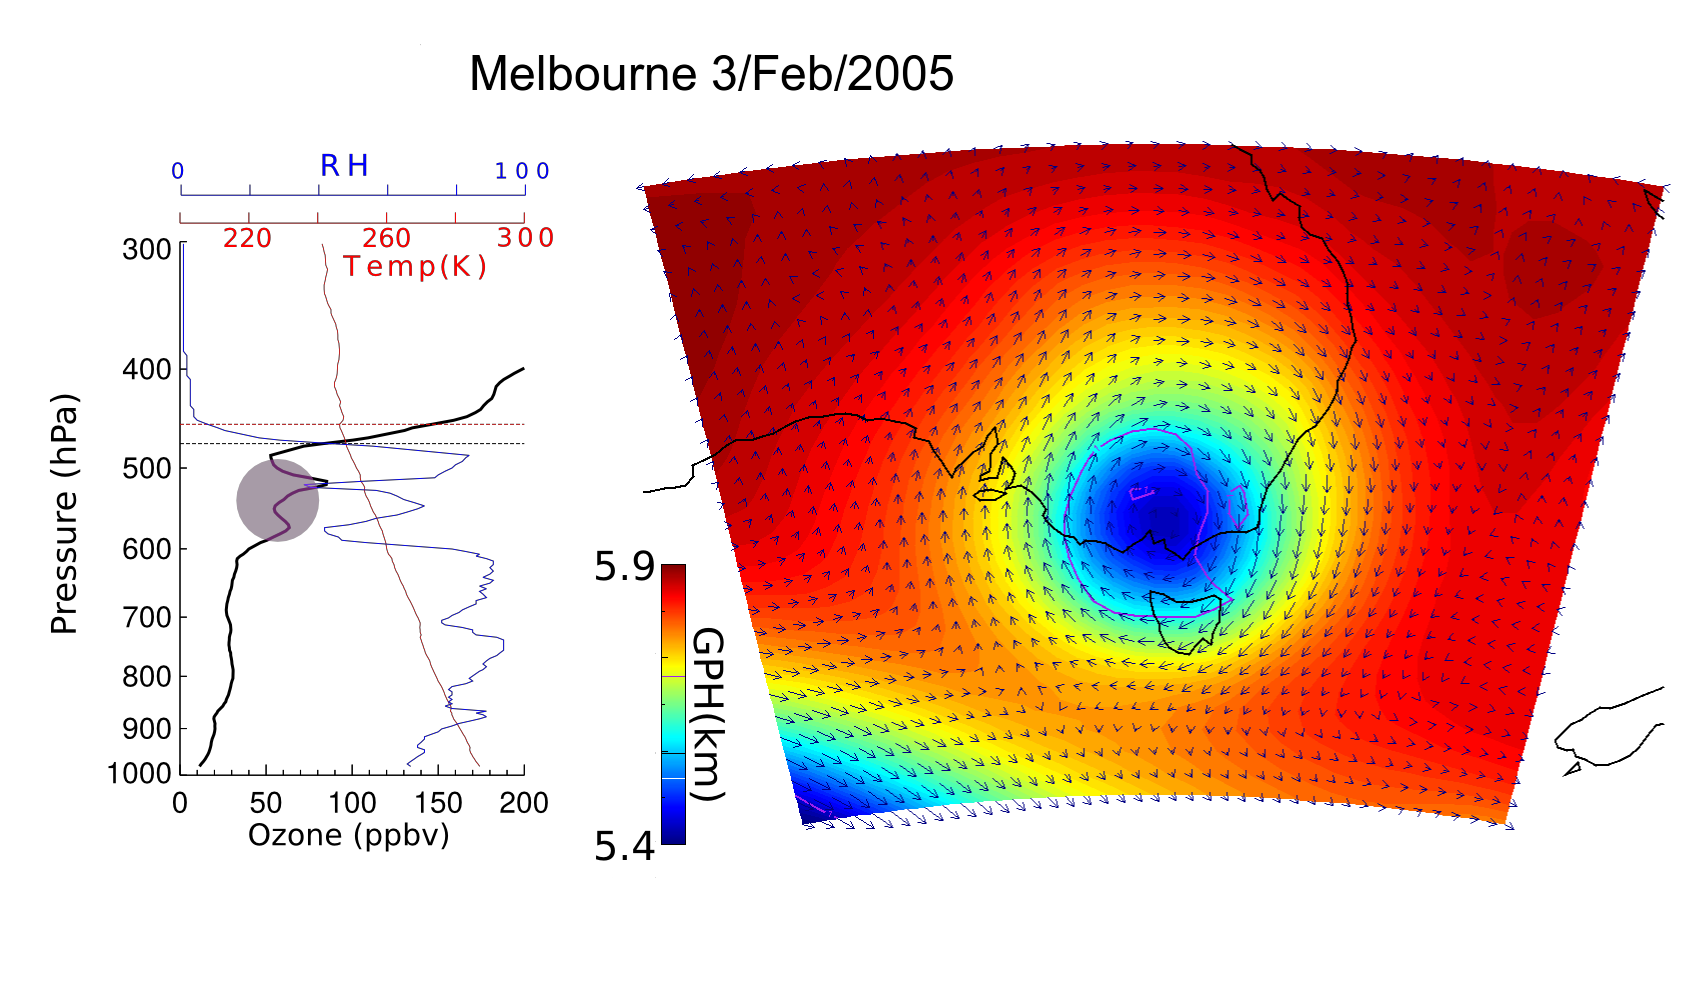
\includegraphics[width=14.0cm]{../figures/Melbourne20050203.png}
      \caption{(Left) Vertical profile of ozone (black), relative humidity (blue), and temperature (red) measured by ozonesonde over Melbourne on 3 February 2005.
      The detected ozone STT event is highlighted in pink.
      Tropopause heights using both the ozone definition (black dashed line) and lapse rate definition (red dashed line) are also shown.
      (Right) Geopotential heights at 500~hPa from the ERA-Interim reanalysis, with wind vectors over-plotted.
      Also shown is the 1~PVU contour line (purple).}
      \label{fig:Melbourne20050203}
    \end{figure*}
    
    \begin{figure*}[t]
    % Figure 6 (discussion version)
    % these IMAGE CREATED BY show_profile.py, EDITTED IN INKSCAPE
      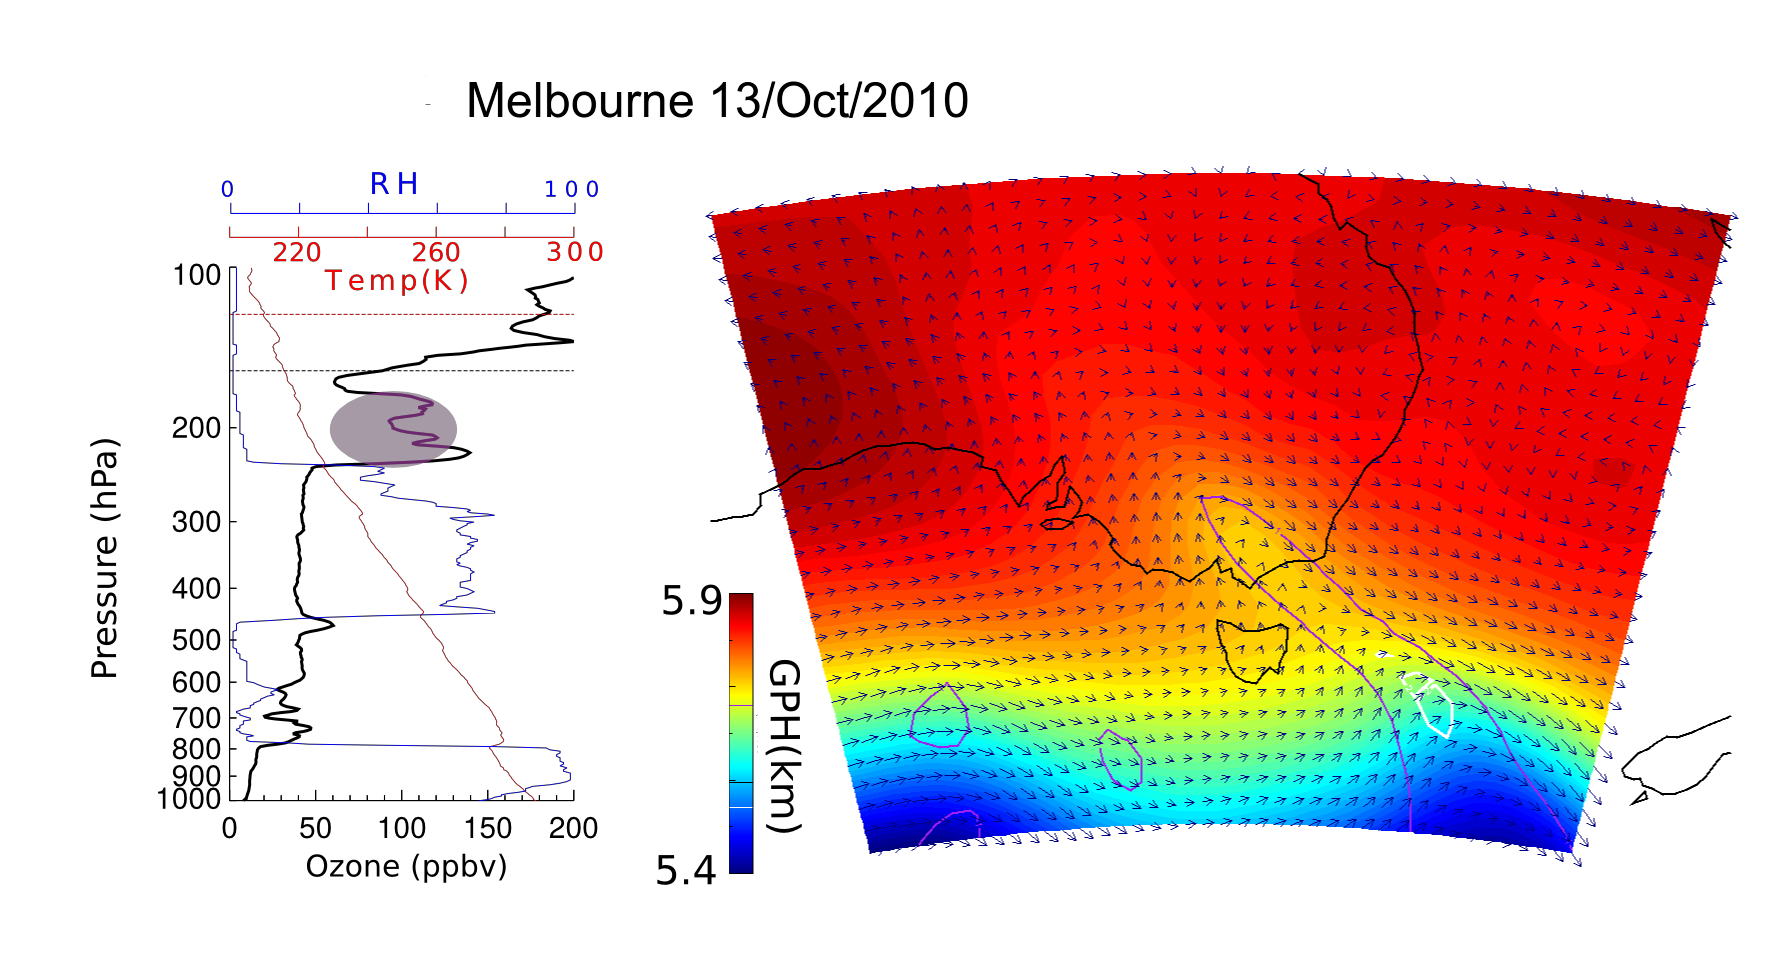
\includegraphics[width=14.0cm]{../figures/Melbourne20100113.png}
      \caption{Same as Fig. \ref{fig:Melbourne20050203} but for 13 January 2010.
	Also shown in this figure is the 2 PVU contour (white), often used to determine dynamical tropopause height.}
      \label{fig:Melbourne20100113}
    \end{figure*}
    
    Figure \ref{fig:Melbourne20050203} (left) shows the vertical ozone profile on 3 February 2005.
    The tropopause was between 400 and 500~hPa and ozone in the upper troposphere was anticorrelated with relative humidity, suggesting the ozone enhancements are due to dry stratospheric air. 
    An ozone intrusion into the troposphere at $\sim$520~hPa was identified by our detection algorithm.
    The right panel shows the concurrent synoptic weather system, a cut-off low pressure system that caused a large storm and lowered the local tropopause height for several days.
    %These systems also increase turbulence near the tropopause, which can lead to increased transport events.
    %The wind circles around the low pressure system in a clockwise direction, typical geostrophic flows which are caused by pressure gradients and coriolis forces.
    The flux of stratospheric ozone into the troposphere associated with this event, calculated using the method shown in Sect. 2.3 of the parent document, was at least $3.1 \times 10^{11}$ molecules cm$^{-3}$, or 8\% of the tropospheric ozone column.
    
    Figure \ref{fig:Melbourne20100113} (left) shows the ozone profile over Melbourne on 13 January 2010.
    The tropopause was higher on this date (120-160~hPa).
    Using our algorithm, we detected an ozone intrusion centred around 200~hPa.
    As before, ozone anti-correlation with relative humidity provides further evidence that the elevated ozone was stratospheric in origin.
    In this profile, there was clear separation between the detected intrusion (highlighted in pink) and the ozone tropopause (black dashed line), which indicates that the sonde passed through regular tropospheric air after hitting a stratospheric intrusion but before reaching the tropopause.
    The right panel shows that this event was associated with a trough (front) of low pressure passing over south eastern Australia.
    This front travelled from west to east and caused a wave of lowered tropopause height. 
    Frontal passage is a known cause of STT as stratospheric air descends and streamers of ozone-rich air break off and mix into the troposphere \citep{Sprenger2003}.
    
\section{Southern Ocean extrapolation}
  \label{sec:SOExtrapolation}

  \subsection{Outline}
    We use simulated tropospheric ozone columns from GEOS-Chem to extrapolate the ozonesonde-based estimates over a large area of the Southern Ocean encompassing our three measurement sites. 
    Figure \ref{fig:SORegion} shows the region defined by latitudes 79$^{\circ}$ - 28$^{\circ}$ S, and longitudes 53$^{\circ}$ - 175$^{\circ}$ E.
    
    \begin{figure}[t]
      % Plot from examine_stations.py in stations repo
      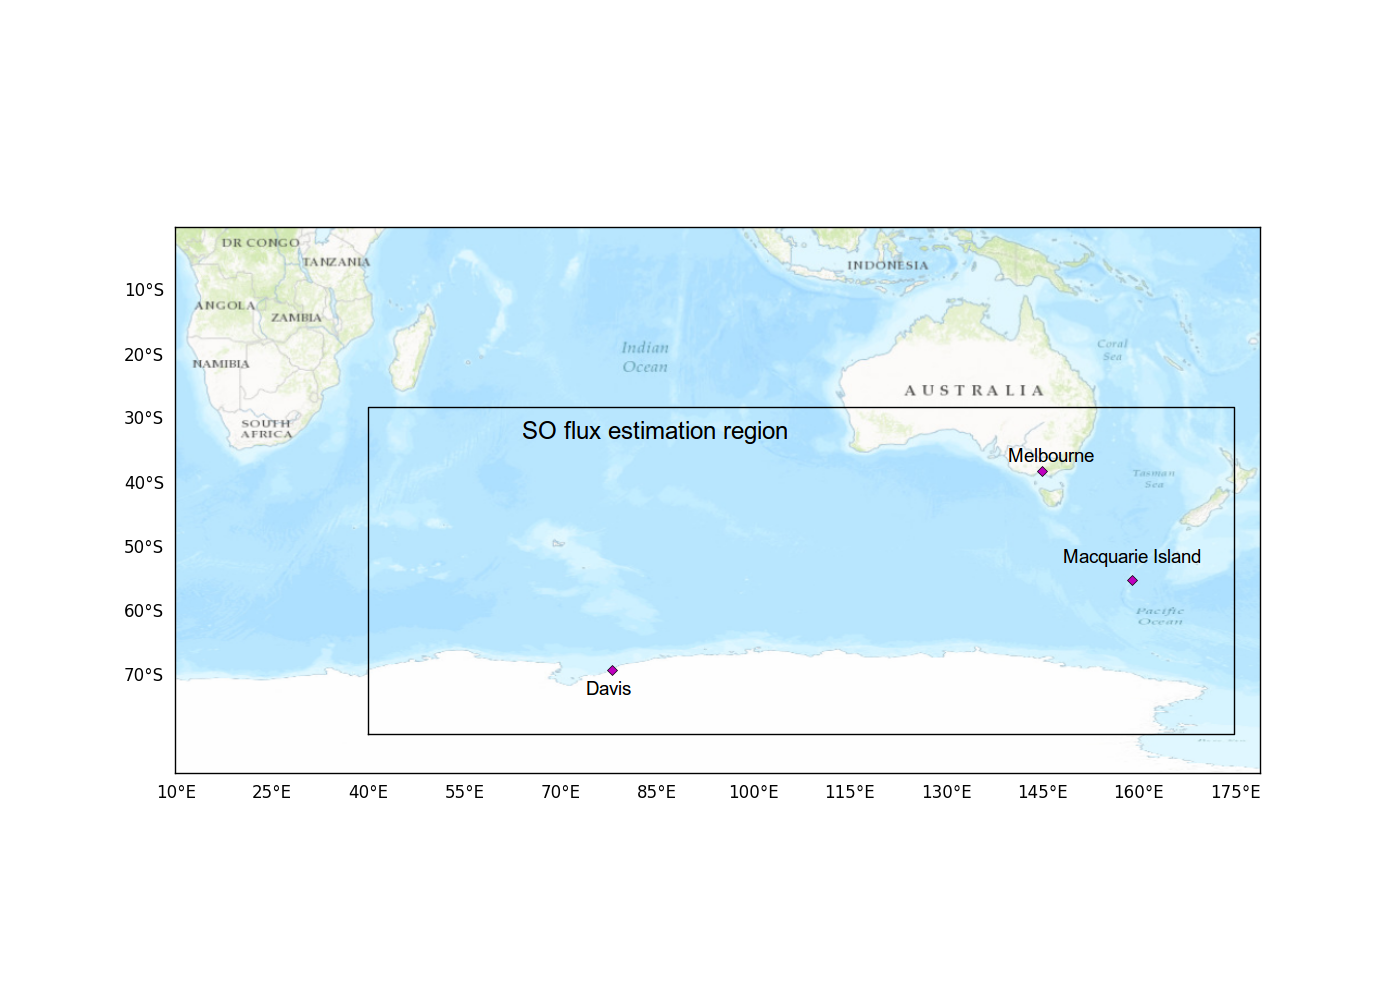
\includegraphics[width=12.0cm]{../figures/OzoneSORegion.png}
      \caption{%
	Region used for large SO estimation of STT flux}
      \label{fig:SORegion}
    \end{figure}
    
    Figure \ref{fig:SOExtrapolation} (upper panel) shows the factors I, P, and $\Omega_{O_3}$ which are used along with the assumed event lifetime to estimate the STT flux.
    The tropospheric ozone and area of our region is calculated using the output and surface area from GEOS-Chem over the Southern Ocean grid boxes along with the molecules cm$^{-2}$ per month calculations, along with ozone molar mass of 48~g mol$^{-1}$.
    
    It is worth noting that this extrapolation is very simplistic and is performed as an example of how the seasonal ozone STT calculations could be used.
    A more spatially resolved estimate could be determined by dividing the Southern Ocean region into longitudinal and latitudinal bins for calculating the average $\Omega_{O_3}$ from GEOS-Chem, as well as applying latitudinal gradients to $P$ and $I$ based on their values at the three sonde release sites, and adding longitudinal variability based on seasonal stratospheric wind jet streams \citep{Baray2012, Skerlak2015}.
    An improved estimate of event lifetime and parameterisation of how many events may be occuring simultaneously could also be addressed, however this is beyond the scope of this work and in any case would not address all the limitations of the estimate provided below.
  \subsection{Results}
    
    Fig. \ref{fig:SOExtrapolation} (lower panel) shows the results of the calculation when we choose two days for our flux estimation, with the range shown in representing the values calculated if we assume events last one day (upper bound of estimated flux) or one week (lower bound of estimated flux).
    Previous studies have found STT ozone fluxes in the SH extratropics are largest from autumn or winter to early spring \citep{Olsen2003, Skerlak2015, Liu2016}.
    Although these are based on dominating STT systems further north than the area we examine here, see the main text for more details.
    During the SH winter, we find the highest tropospheric $\Omega_{O3}$ but a relatively low STT flux due to reduced event frequency.
    Our results suggest instead that the ozone flux associated with STT events (at least those due to tropopause folds) is largest in austral summer (December-March), primarily due to an increased frequency of STT detections during these months.
    It is possible that our estimated event frequencies are too low in late winter-early spring as some legitimate STT events may have been excluded due to coincident smoke plumes.
    
    \begin{figure}[t]
      % Plot from examine_stations.py in stations repo
      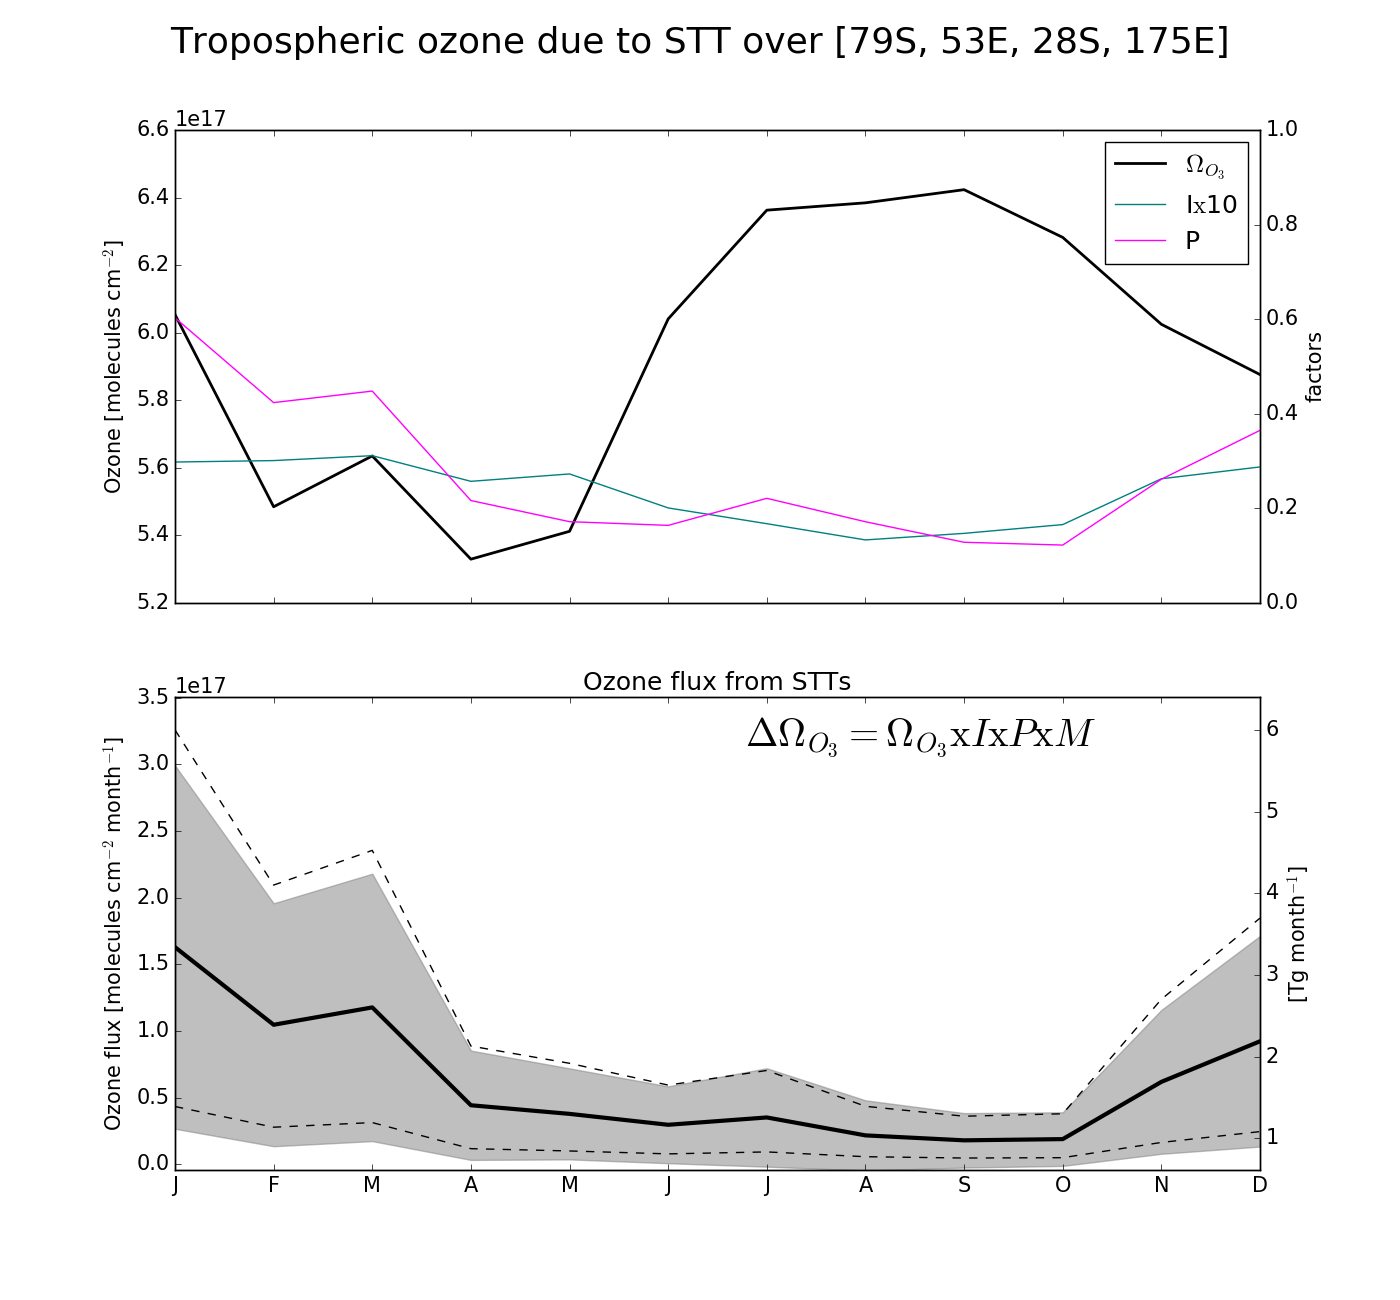
\includegraphics[width=12.0cm]{../figures/STT_extrapolation_SO.png}
      \caption{%
	(Top) The three quantities used to calculate the total Southern Ocean ozone flux from STT events.
	The tropospheric ozone column $\Omega_{O_3}$ (black, left axis) is from GEOS-Chem, while the STT probability $P$ (magenta, right axis) and impact $I$ (teal, right axis) are from the ozonesonde measurements.
	The STT impact is multiplied by 10 to better show the seasonality.
	(Bottom) Estimated contribution of STT to tropospheric ozone columns over the Southern Ocean.
	The shaded area shows the uncertainty as calculated in Sect. 6 of the parent document, with the -dashed lines showing the range of values when assuming events last one day (upper dashed line) up to one week (lower dashed line).}
      \label{fig:SOExtrapolation}
    \end{figure}
    
    Summing the monthly estimated fluxes shown in Fig. \ref{fig:SOExtrapolation} over the year, we find from this estimate that STT events may be responsible for $\sim 7.5 \times10^{16}$~molecules cm$^{-2}$ yr$^{-1}$ of the tropospheric ozone over the Southern Ocean, equivalent to 75~Tg yr$^{-1}$.
    $2$-$16 \times 10^{16}$ molecules cm$^{-2}$ of stratospheric based ozone is estimated over the southern ocean throughout the year.
    Our estimate is hard to directly compare to prior work that suggests global gross STT fluxes of 550~Tg yr$^{-1}$ \citep{Stevenson2006} and net downward STT fluxes of 75~Tg yr$^{-1}$ \citep{Sprenger2003}.
    This is due to the high uncertainties involved in calculation as well as the specific regions which have few other measurements available.

% not putting this in as simon say's it's kiddies stuff
%\section{Fast fourier transform code (IDL)}
%\label{sec:FFTCode}
% Provided by Dr. Simon Alexander.
% 
%\verbatiminput{sa_filter_1d.pro}

\bibliographystyle{copernicus}
\bibliography{bibliography/Ozone.bib}

\end{document}
